%iffalse
\let\negmedspace\undefined
\let\negthickspace\undefined
\documentclass[journal,12pt,onecolumn]{IEEEtran}
\usepackage{cite}
\usepackage{amsmath,amssymb,amsfonts,amsthm}
\usepackage{algorithmic}
\usepackage{graphicx}
\usepackage{textcomp}
\usepackage{xcolor}
\usepackage{txfonts}
\usepackage{listings}
\usepackage{enumitem}
\usepackage{mathtools}
\usepackage{gensymb}
\usepackage{comment}
\usepackage[breaklinks=true]{hyperref}
\usepackage{tkz-euclide} 
\usepackage{listings}
\usepackage{gvv}                                        
%\def\inputGnumericTable{}                                 
\usepackage[latin1]{inputenc}                                
\usepackage{color}                                            
\usepackage{array}                                            
\usepackage{longtable}                                       
\usepackage{calc}                                             
\usepackage{multirow}                                         
\usepackage{hhline}                                           
\usepackage{ifthen}                                           
\usepackage{lscape}
\usepackage{tabularx}
\usepackage{array}
\usepackage{float}
\usepackage{multicol}
\usepackage{subcaption}

\newtheorem{theorem}{Theorem}[section]
\newtheorem{problem}{Problem}
\newtheorem{proposition}{Proposition}[section]
\newtheorem{lemma}{Lemma}[section]
\newtheorem{corollary}[theorem]{Corollary}
\newtheorem{example}{Example}[section]
\newtheorem{definition}[problem]{Definition}
\newcommand{\BEQA}{\begin{eqnarray}}
\newcommand{\EEQA}{\end{eqnarray}}
\newcommand{\define}{\stackrel{\triangle}{=}}
\theoremstyle{remark}
\newtheorem{rem}{Remark}


% Marks the beginning of the document
\begin{document}
\bibliographystyle{IEEEtran}
\vspace{3cm}

\title{NCERT-10.4.3.3.1}
\author{S. Sai Akshita - EE24BTECH11054}
\newpage
\maketitle
\bigskip

\renewcommand{\thefigure}{\theenumi}
\renewcommand{\thetable}{\theenumi}
\textbf{Question:} 
Find the roots of the following Equation:
\begin{align}
    x-\frac{1}{x} =3, x\neq 0 \label{eq.1}
\end{align}
\textbf{Theoretical Solution:}
To eliminate the fraction, multiply \ref{eq.1} through by $x$ (valid because $ x \neq 0 $):
\begin{align}
x^2 - 1 = 3x.
\end{align}
Rearranging terms gives the quadratic equation:
\begin{align}
f\brak{x}=x^2 - 3x - 1 = 0.\label{qe}
\end{align}
Comparing this with the following equation:
\begin{align}
    ax^2+bx+c=0
\end{align}
We get $a=1,b=-3,c=-1$.\\
We solve this quadratic equation using the quadratic formula:
\begin{align}
x = \frac{-b \pm \sqrt{b^2 - 4ac}}{2a},
\end{align}
Substituting the values:
\begin{align}
x = \frac{-(-3) \pm \sqrt{(-3)^2 - 4(1)(-1)}}{2(1)}.
\end{align}
Simplify the expression:
\begin{align}
x &= \frac{3 \pm \sqrt{9 + 4}}{2}\\
x &= \frac{3 \pm \sqrt{13}}{2}.
\end{align}
Thus, the solutions are:
\begin{align}
\alpha = \frac{3 + \sqrt{13}}{2} \quad \approx 3.3028 \text{and} \quad \beta = \frac{3 - \sqrt{13}}{2}\approx -0.3028.
\end{align}
Since $ x \neq 0 $, both solutions are valid.\\
\textbf{Solution by using Newton-Raphson method:}
To apply the Newton-Raphson method, we use the iterative formula:
\begin{align}
	x_{n+1} = x_n - \frac{f\brak{x_n}}{f^\prime\brak{x_n}},\label{nrm1}
\end{align}
where $ f^\prime\brak{x} $ is the derivative of $f\brak{x} $.
The derivative of $f\brak{x}$ is:
\begin{align}
f^\prime\brak{x} = 2x-3.
\end{align}
Substituting in \ref{nrm1}, The iterative formula becomes:
\begin{align}
x_{n+1} = x_n - \frac{{x_n}^2 - 3x_n - 1 }{2x_n-3}.\label{nrm}
\end{align}
For the iterative process, choose an initial guess $ x_0 $. Then substitute it in \ref{nrm} to obtain $x_1,x_2,$ and so on until the value of $\epsilon$ is greater than that of $ \lvert x_{n+1} - x_n\rvert $. Here, $\epsilon$ should be allotted a smaller value for better precision of the roots.\\
The Newton-Raphson method provides an efficient way to numerically approximate the solution. Iterative computation can be performed using a program to find the root up to the desired precision. For the graph obtained, initial guess are $4$ and $0.5$, and $\epsilon=0.000001$.Roots obtained through iteration are $\alpha=3.3027756377328092,\beta=-0.30277563792072887.$\\
\textbf{Fixed Point Iteration:}
The given equation is \ref{eq.1}\\
To apply the Fixed-Point Iteration Method, we rewrite the equation in the form:
\begin{align}
x = g\brak{x}.\label{fim}
\end{align}
Possible rearrangements are:
\begin{align}
x &= \frac{1}{x} + 3.\\
x&= \frac{x^2 -1}{3}
\end{align}
The iterative formulas are:
\begin{align}
x_{\brak{n+1}1} &= \frac{1}{x_n} + 3\\
x_{\brak{n+1}2} &= \frac{x_n^2 -1}{3}.
\end{align}
Choose an initial guess $x_0$. Continue the process until the difference between consecutive approximations $ \lvert x_{n+1} - x_n\rvert $ is smaller than the desired tolerance $\epsilon$. The convergence of the Fixed-Point Iteration depends on the choice of $ g\brak{x} $. \\\\
\textbf{Steffensen's Method (Quadratic Convergence):}
Steffensen's method accelerates the convergence of fixed-point iteration. If $ g\brak{x} $ is the iteration function derived from the fixed-point form of $ f\brak{x} $, Steffensen's iterative formula is:
\begin{align}
x_{n+1} = x_n - \frac{g\brak{x_n}}{\frac{g\brak{x_n+g\brak{x_n}}}{g\brak{x_n}}-1} \label{sif}
\end{align}
This eliminates the need to compute derivatives and achieves quadratic convergence.\\Rewrite the equation in the fixed-point form, i.e., \ref{fim}.\\
For this problem,they are:
\begin{align}
g_1\brak{x_n} &= \frac{1}{x_n} + 3.\\
g_2\brak{x_n} &= \frac{x_n^2-1}{3}.
\end{align}
Substitute in \ref{sif}
\begin{align}
x_{\brak{n+1}1}&=x_n^2+4x_n+1\\
x_{\brak{n+1}2}&=x_n -\frac{\brak{x_n^2-1}^2}{\brak{x_n^2+3x_n-1}^2-9x_n^2}
\end{align}
Continue iterating until $ \lvert x_{n+1} - x_n\rvert < \epsilon $, where $ \epsilon $ is the desired accuracy.
Steffensen's method converges quadratically under suitable conditions, making it significantly faster than standard fixed-point iteration.
\textbf{Solution using QR Algorithm:} 
A quadratic equation is given by:
\begin{align}
 ax^2 + bx + c = 0   
\end{align}
To construct the companion matrix, normalize the equation ($a \neq 0$) by dividing through by $a$:
\begin{align}
x^2 + \frac{b}{a}x + \frac{c}{a} = 0
\end{align}
The companion matrix for the quadratic equation is:
\begin{align}
C = \begin{bmatrix}
0 & -\frac{c}{a} \\
1 & -\frac{b}{a}
\end{bmatrix}
\end{align}
For \ref{qe}, it is:
\begin{align}
C = \begin{bmatrix}
0 & 1 \\
1 & 3
\end{bmatrix}
\end{align}
The eigenvalues of the companion matrix $C$ are the roots of the quadratic equation. The goal is to use the QR algorithm to approximate the eigenvalues of $C$. The steps are as follows:
\begin{enumerate}
    \item Start with the matrix $C$:
    \begin{align}
    C = \begin{bmatrix}
    0 & 1 \\
    1 & 3
    \end{bmatrix}.
    \end{align}

    \item Perform QR decomposition:
    Factor $C$ into:
    \begin{align}
    C = QR,
    \end{align}
    where:
    \begin{itemize}
        \item $Q$ is an orthogonal matrix ($Q^T Q = I$),
        \item $R$ is an upper triangular matrix.
    \end{itemize}

    \item Update the matrix:
    Compute:
    \begin{align}
    C_{k+1} = RQ.
    \end{align}

    \item Iterate:
    Repeat the QR decomposition and update step until $C_k$ converges to an upper triangular matrix. The diagonal entries of the resulting matrix are the eigenvalues of $C$.
\end{enumerate}
By using the QR Decomposition, the eigenvalues,i.e., the roots obtained are
\begin{align}
    \alpha&=3.30277564\\
    \beta&=-0.30277564
\end{align}

\begin{figure}[h] % 'h' means place the image here
    \centering % Centers the image
    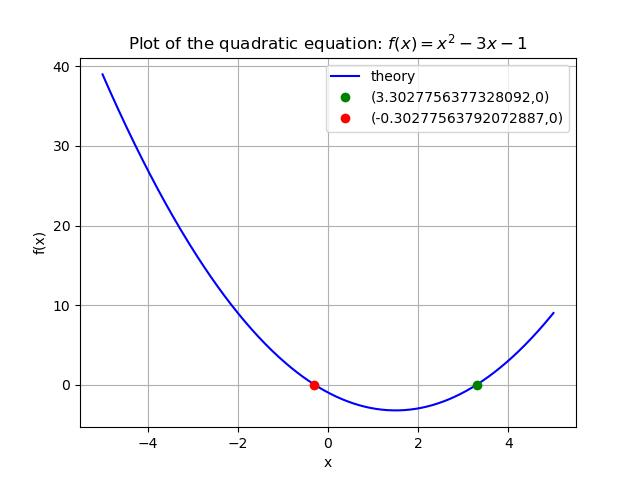
\includegraphics[width=0.5\columnwidth]{figs/Newton-Raphson.jpeg} % Adjust width as needed
    \label{fig:example_image} % Reference label for the image
\end{figure}

\begin{figure}[h] % 'h' means place the image here
    \centering % Centers the image
    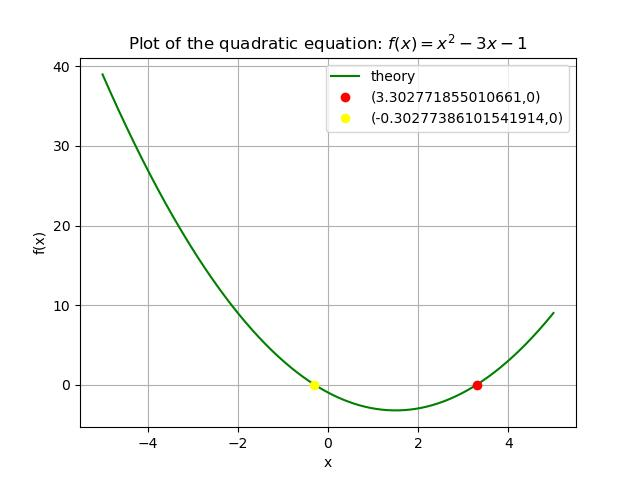
\includegraphics[width=0.5\columnwidth]{figs/fpi.jpeg} % Adjust width as needed
    \label{fig:example_image} % Reference label for the image
\end{figure}

\begin{figure}[h] % 'h' means place the image here
    \centering % Centers the image
    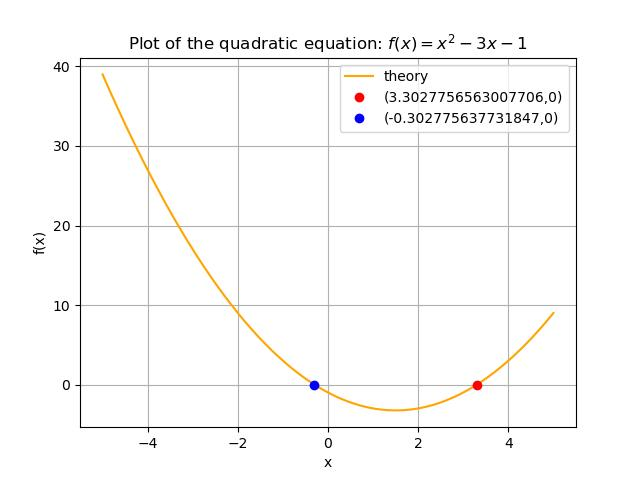
\includegraphics[width=0.5\columnwidth]{figs/steffenson.jpeg} % Adjust width as needed
    \label{fig:example_image} % Reference label for the image
\end{figure}



\end{document}
